\begin{center}
  \section*{Homework 06 - 3.4}
  Due Mar 20 \\
  Uzair Hamed Mohammed
\end{center}

% 6, 9, 14

\begin{enumerate}
  \item[6.] Let n be a positive integer. Show that \(f_Y(y) = (n + 2)
    (n + 1) y^n (1 - y), 0 \leq y \leq 1\), is a pdf.

    \underline{Sol}:\\

    \[
      n \in \mathbb{Z}^+, y \in [0, 1] \implies (n + 2) (n + 1) > 0,
      y^n \ge 0, (1 - y) \ge 0
    \]

    \[
      \begin{aligned}
        \int_{0}^{1} (n+2)(n+1)y^n(1-y) dy &= (n+2)(n+1) \int_{0}^{1}
        (y^n - y^{n+1}) dy \\
        &= (n+2)(n+1) \left[ \frac{y^{n+1}}{n+1} -
        \frac{y^{n+2}}{n+2} \right]_0^1 \\
        &= (n+2)(n+1) \left( \frac{1}{n+1} - \frac{1}{n+2} \right) \\
        &= (n+2)(n+1) \left[ \frac{(n+2) - (n+1)}{(n+1)(n+2)} \right] \\
        &= \frac{(n+2)(n+1)}{(n+1)(n+2)} \\
        &= 1
      \end{aligned}
    \]

  \item[9.] If the pdf for \(Y\) is
    \begin{equation*}
      f_Y(y) =
      \begin{cases}
        0, & |y| > 1 \\
        1 - |y|, & |y| \leq 1
      \end{cases}
    \end{equation*}

    find and graph \(F_Y(y)\).

    \underline{Sol}:\\

    $$F_Y(y) = \int_{-\infty}^y f_Y(t) dt$$
    For \(y < -1\):
    \[F_Y(y) = 0\]
    For \(-1 \le y < 0\):
    \[F_Y(y) = \int_{-1}^y (1+t) dt = \left[ t + \frac{t^2}{2}
      \right]_{-1}^y = (y + \frac{y^2}{2}) - (-1 + \frac{1}{2}) =
    \frac{1}{2}(y+1)^2\]
    For \(0 \le y \le 1\):
    \[F_Y(y) = F_Y(0) + \int_0^y (1-t) dt = \frac{1}{2} + \left[ t -
      \frac{t^2}{2} \right]_0^y = \frac{1}{2} + y - \frac{y^2}{2} = 1 -
    \frac{1}{2}(1-y)^2\]
    For \(y > 1\):
    \[F_Y(y) = 1\]
    \[F_Y(y) =
      \begin{cases} 0, & y < -1 \\ \frac{1}{2}(y+1)^2, & -1 \le y < 0
        \\ 1 - \frac{1}{2}(1-y)^2, & 0 \le y \le 1 \\ 1, & y > 1
    \end{cases}\]

    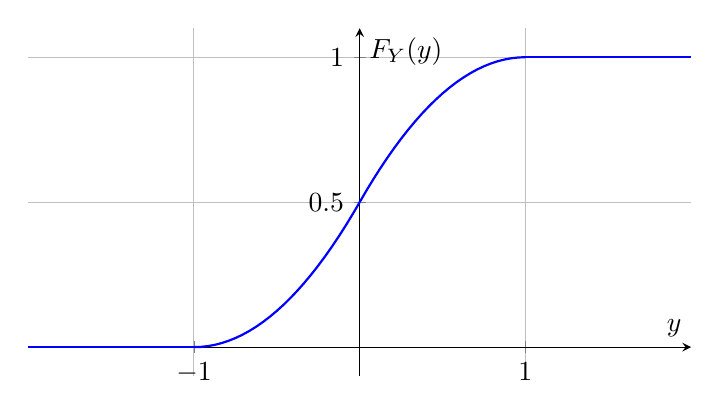
\begin{tikzpicture}
      \begin{axis}[
          axis lines = middle,
          xlabel = $y$,
          ylabel = {$F_Y(y)$},
          xmin = -2, xmax = 2,
          ymin = -0.1, ymax = 1.1,
          ytick = {0, 0.5, 1},
          xtick = {-1, 0, 1},
          grid = both,
          width=10cm, height=6cm
        ]
        \addplot [domain=-2:-1, blue, thick] {0};
        \addplot [domain=-1:0, blue, thick] {0.5*(x+1)^2};
        \addplot [domain=0:1, blue, thick] {1 - 0.5*(1-x)^2};
        \addplot [domain=1:2, blue, thick] {1};
      \end{axis}
    \end{tikzpicture}

  \item[14.] In a certain country, the distribution of a family's
    disposable income, \(Y\), is described by the pdf \(f_Y(y) =
    ye^{-y}, y \geq 0\). Find \(F_Y(y)\).

    \underline{Sol}:\\

    \[F_Y(y) = \int_{0}^{y} f_Y(t) dt = \int_{0}^{y} t e^{-t} dt\]

    Integration by parts: Let \(u = t, dv = e^{-t} dt \implies du =
    dt, v = -e^{-t}\)

    \[\int t e^{-t} dt = -t e^{-t} - \int -e^{-t} dt = -t e^{-t} -
    e^{-t} = -(t+1)e^{-t}\]

    Evaluating the definite integral:

    \[F_Y(y) = \left[ -(t+1)e^{-t} \right]_0^y\]

    \[F_Y(y) = -(y+1)e^{-y} - (-(0+1)e^0)\]

    \[F_Y(y) = 1 - (y+1)e^{-y}, \quad y \ge 0\]

    For \(y < 0$, $F_Y(y) = 0\).

    \[F_Y(y) =
      \begin{cases} 1 - (y+1)e^{-y}, & y \ge 0 \\ 0, & y < 0
    \end{cases}\]
\end{enumerate}
